\documentclass[10pt,aspectratio=169, colorlinks=true, linkcolor=circlBlue]{beamer}

% tlp allowed values: clear, green, amber, amber+strict, red
\usetheme[numbering=fraction, progressbar=frametitle, tlp=clear]{circl}

% for code highlighting
\usepackage{minted}
% to draw pingus
\usepackage{tikzpingus}
% to draw boxes to catch attention
\usepackage{awesomebox}
% For hyperlinks in the document and PDF metadata
\usepackage{hyperref}
% useful only if we want to customize minted background
\usepackage{tcolorbox}

\usepackage{multicol}
%
% compile with -shell-escape in order to use minted
% $ pdflatex  -interaction=nonstopmode -shell-escape presentation.tex
%


\hypersetup{
    pdftitle={The Art of Pivoting - How You Can Discover More from Adversaries with Existing Information},    % Title
    pdfauthor={Alexandre Dulaunoy, Aurelien Thirion},               % Author
    pdfsubject={The Art of Pivoting - How You Can Discover More from Adversaries with Existing Information}, % Subject
    pdfkeywords={AIL Project, Art of Pivoting, CTI, Threat Intelligence}, % Keywords
    colorlinks=false,                       % Color links instead of boxes
    linkcolor=blue,                        % Color of internal links
    citecolor=blue,                        % Color of citations
    urlcolor=blue                          % Color of external links
}

% set the logo to put in the title page
\titlegraphic{\noindent\hfill
\includegraphics[width=0.25\textwidth]{img/logo-circl.pdf}}
\title{The Art of Pivoting - How You Can Discover More from Adversaries with Existing Information}
\subtitle{CIRCL - Virtual Summer School 2025}
\date{July 17, 2025}
\author{Alexandre Dulaunoy - alexandre.dulaunoy@circl.lu / Aurelien Thirion - aurelien.thirion@circl.lu}
\institute{CIRCL \normalurl{https://www.circl.lu}}
% if set inserts a title link into the title page
\titlelink{\faHome\space \normalurl{https://www.ail-project.org}}

\begin{document}

% include custom commands

% Place here your custom commands, it will be included in presentation.tex

\newcommand{\normalurl}[1]{\href{#1}{#1}}

\newcommand{\footnoteurl}[1]{\footnote{\scriptsize\url{#1}}}

\newcommand{\rocketbox}[1]{%
	\awesomebox[circlRed]{1pt}{\faRocket}{circlBlue}{#1}%
}


% Title page
\begin{frame}
	\titlepage%
\end{frame}


% --------- Summary ---------
%\setcounter{tocdepth}{2}
%\begin{frame}
%    \frametitle{Content at glance}
%    \tableofcontents
%\end{frame}
%\setcounter{tocdepth}{4}
% ----------------------------


\begin{frame}
    \frametitle{What is Defender's Pivoting?}
    \begin{itemize}
	    \item Pivoting\footnote{The term “pivoting” can cause confusion. In this context, we refer to defender's pivoting using data points, distinct from the threat actor's lateral movement within a compromised infrastructure.} is the analytical process of using one known artifact (such as an indicator of compromise (IOC), behavioral fingerprint, or identity trace) to uncover additional, related elements within a threat actor’s infrastructure, toolkit, service, or operation. This technique enables analysts to expand the scope of an investigation, uncover hidden connections, confirm or attribute activity, and anticipate future adversary behavior.
    \end{itemize}
\end{frame}

\begin{frame}
    \frametitle{Six Degrees of Separation and Pivoting}
    \begin{itemize}
        \item The concept of \textit{six degrees of separation}\footnote{Also referenced in popular culture as the "Six Degrees of Kevin Bacon," or in academic contexts as the "Erdős number," which measures how many co-authorship links separate a researcher from mathematician Paul Erdős.} suggests that any two individuals are connected through a chain of six or fewer social relationships.
        \item Similarly, in threat intelligence, pivoting is an analyst's method for uncovering hidden relationships, much like navigating a social graph. Instead of people, we’re connecting data points and observables.
        \item Just as social networks reveal how people are linked, threat intelligence graphs reveal how indicators, infrastructure, and behaviors are interrelated, enabling defenders to map out and understand adversary ecosystems.
    \end{itemize}
\end{frame}

\begin{frame}
    \frametitle{Analytical Benefits of Pivoting}
    \begin{columns}
        \begin{column}{0.5\textwidth}
            \begin{itemize}
                \item {\bf Current:} Understand how a threat actor interacts, communicates, and operates in real time.
                \item {\bf Historical:} Reveal past connections between threat actors and specific infrastructure or identities.
                \item {\bf Predictive:} Anticipate future actions based on recurring patterns, techniques, and operational habits.
            \end{itemize}
        \end{column}
        \begin{column}{0.5\textwidth}
            \centering
            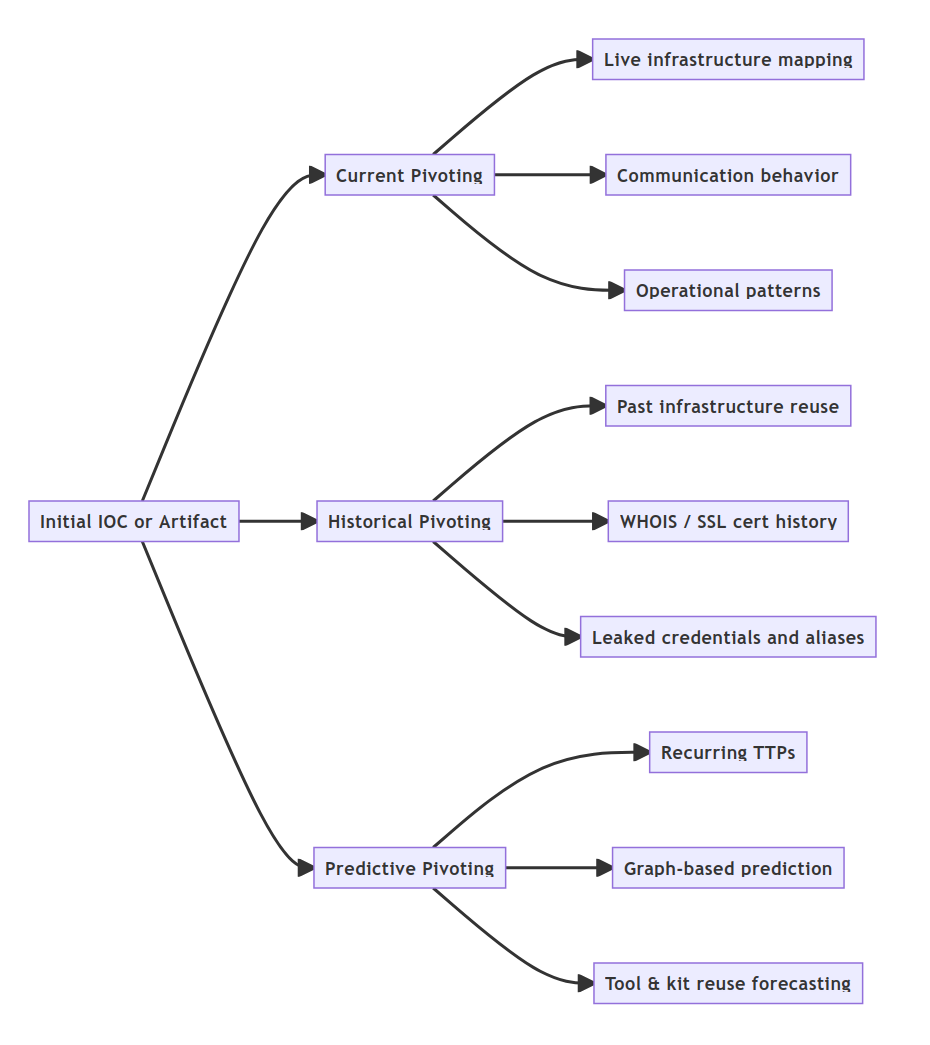
\includegraphics[scale=0.19]{img/pivot-overview.png}
        \end{column}
    \end{columns}
\end{frame}

\begin{frame}
    \frametitle{Is Pivoting Evolving?}
    \begin{itemize}
        \item We strive to shift pivoting from an art to a science, making it reproducible, practical, and truly actionable for analysts.
	\item Yet, our perspective is sometimes clouded by {\bf rigid models} or {\bf legacy practices} that may no longer reflect today’s threat landscape.
        \item Should we reconsider our reliance on models like the \textit{Pyramid of Pain}, and critically assess how difficult it really is for adversaries to alter high-value indicators?
        \item Do threat actors always realize which traces they leave behind\footnote{Remember where the ``Anna-Senpai'' handle eventually led?}, and can they truly gauge the intelligence value of what they expose?
    \end{itemize}
\end{frame}

\begin{frame}
    \frametitle{Re-evaluating Our Indicator Collection and Pivoting Practices}
    \begin{itemize}
        \item In the AIL project\footnote{\url{https://ail-project.org/}}, we collect a wide range of sources—from social networks and Tor hidden services to forums and specific web infrastructure used by threat actors.
        \item We’ve implemented a dynamic correlation engine that allows easy integration of new object types for pivoting and analysis.
	\item This required a mindset shift: {\bf focusing more on outliers and overlooked data points}, while challenging and discarding some of our older assumptions.
    \end{itemize}
\end{frame}

\begin{frame}
    \frametitle{Looking at Broken Indicators—and Still Using Them}

    \begin{itemize}
        \item MurmurHash3 is still widely used for favicon correlation. It enables quick discovery of Tor hidden services exposed on the clear web through simple hash-based pivoting.
	\item If MurmurHash3 is known to be flawed, why do we still use it? Because despite its weaknesses\footnote{The same question can be asked about other algorithms used in threat intelligence processing.}, it remains effective—and threat actors rarely think to modify their favicons.
        \item An interesting angle: some actors may attempt to create hash collisions. Correlating on *colliding* favicons can itself become a pivoting technique. So why stop calculating them?
    \end{itemize}
\end{frame}

\begin{frame}
    \frametitle{Favicons as Differentiators and Composite Correlation Points}
    \begin{columns}
        \begin{column}{0.5\textwidth}
            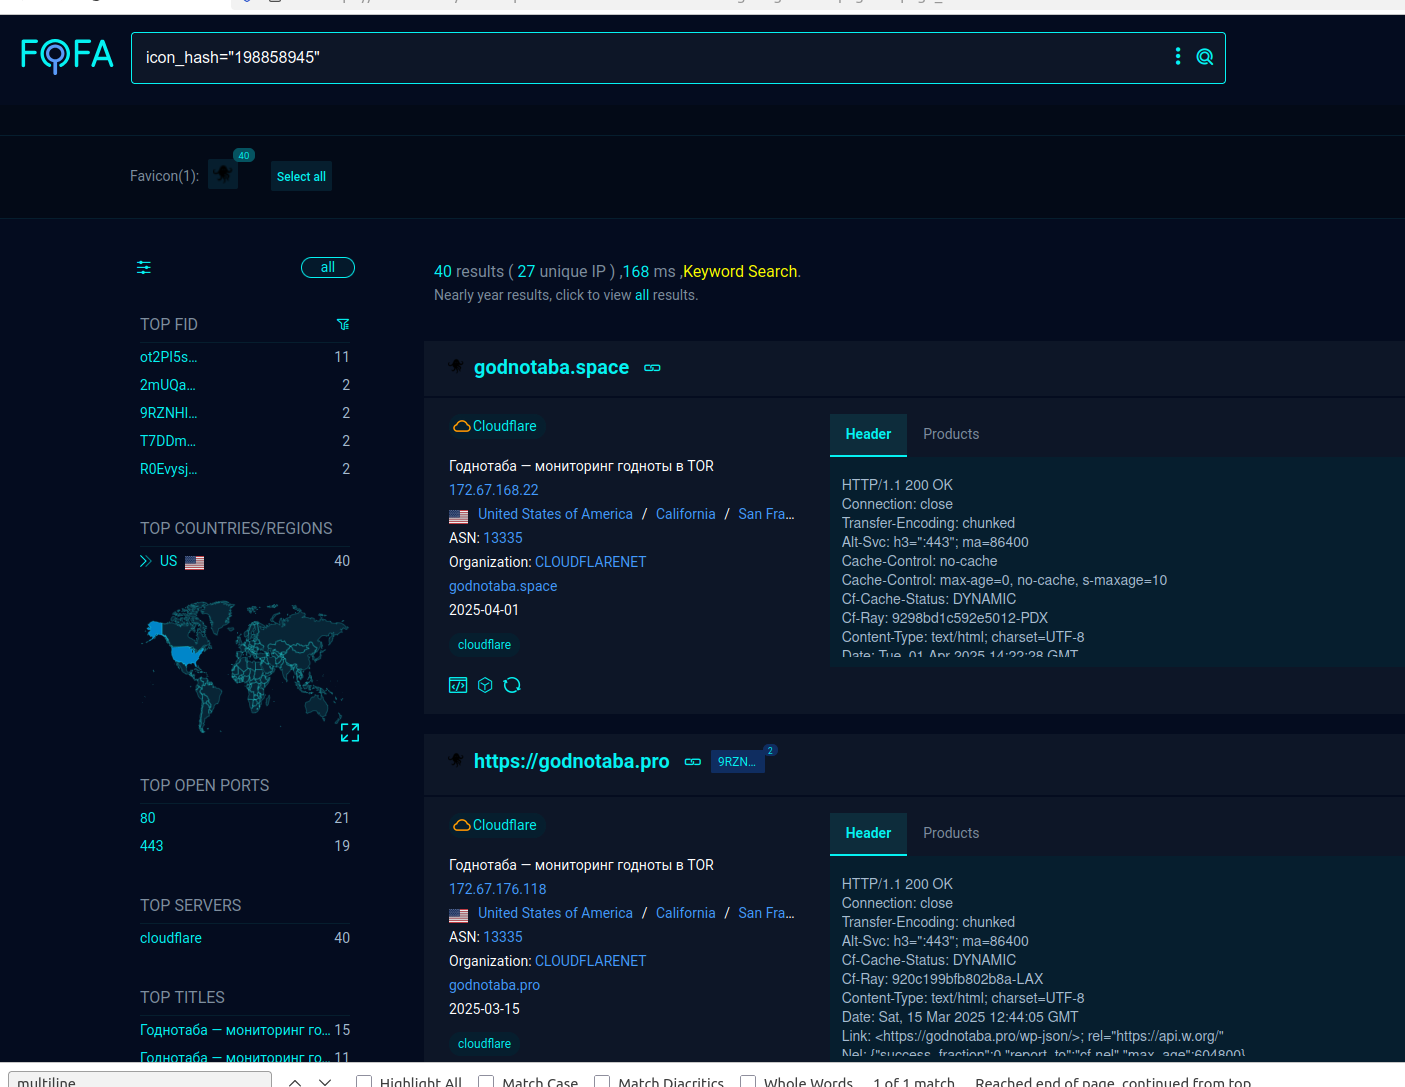
\includegraphics[scale=0.15]{./img/favicon-fofa.png}
        \end{column}
        \begin{column}{0.5\textwidth}
            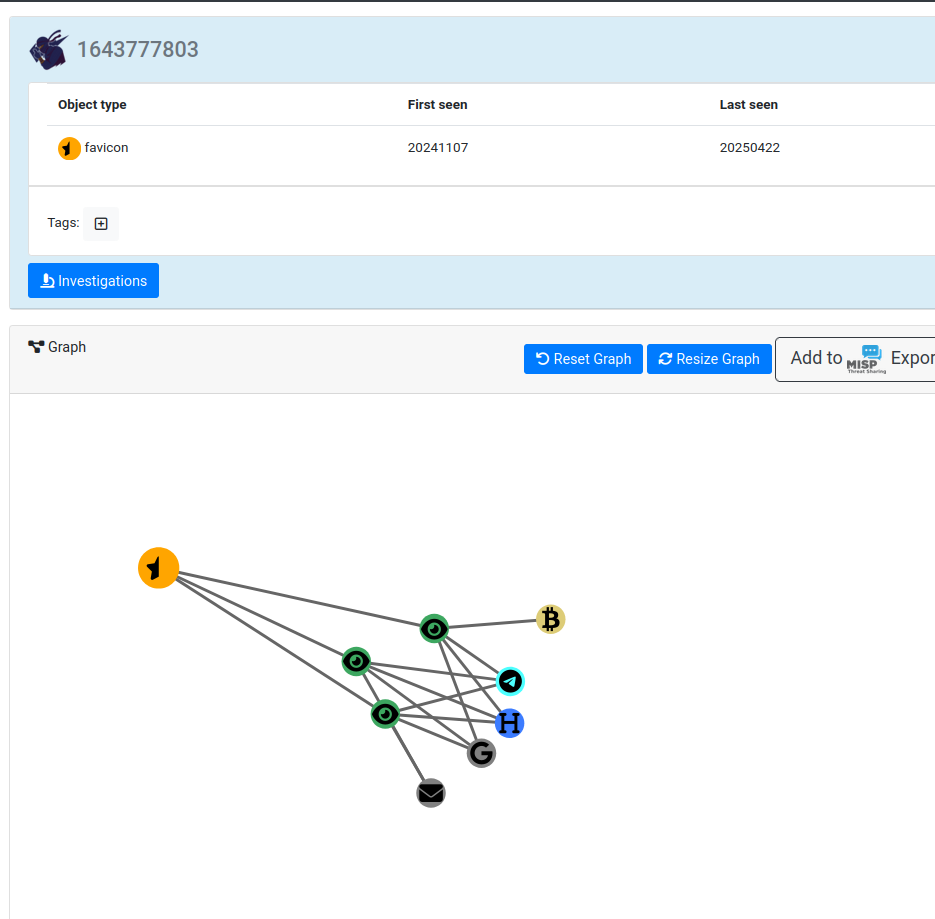
\includegraphics[scale=0.15]{./img/favicon-2.png}
        \end{column}
    \end{columns}
    \vspace{0.5em}
    \begin{center}
        {\small Even seemingly innocuous favicons can act as unique fingerprints—useful for correlating threat infrastructure across campaigns or layers (e.g., Tor vs. clear web).}
    \end{center}
\end{frame}

\begin{frame}
    \frametitle{Uncommon Indicator Extraction: QR Codes}
    \begin{itemize}
        \item QR codes are increasingly seen across social networks, Tor hidden services, and even in ransomware negotiation pages.
    \end{itemize}
    \begin{columns}
        \begin{column}{0.5\textwidth}
            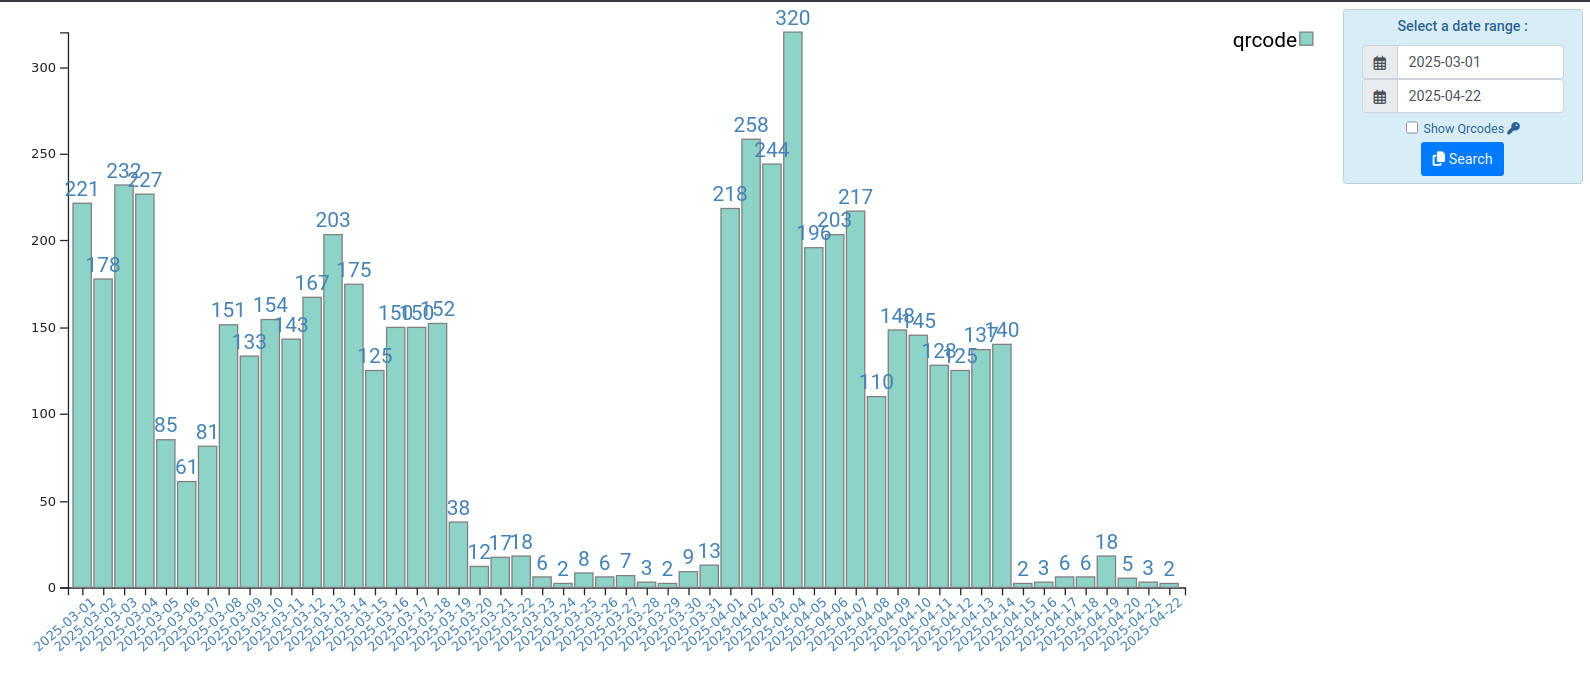
\includegraphics[scale=0.15]{./img/qrcode-2.png}
	    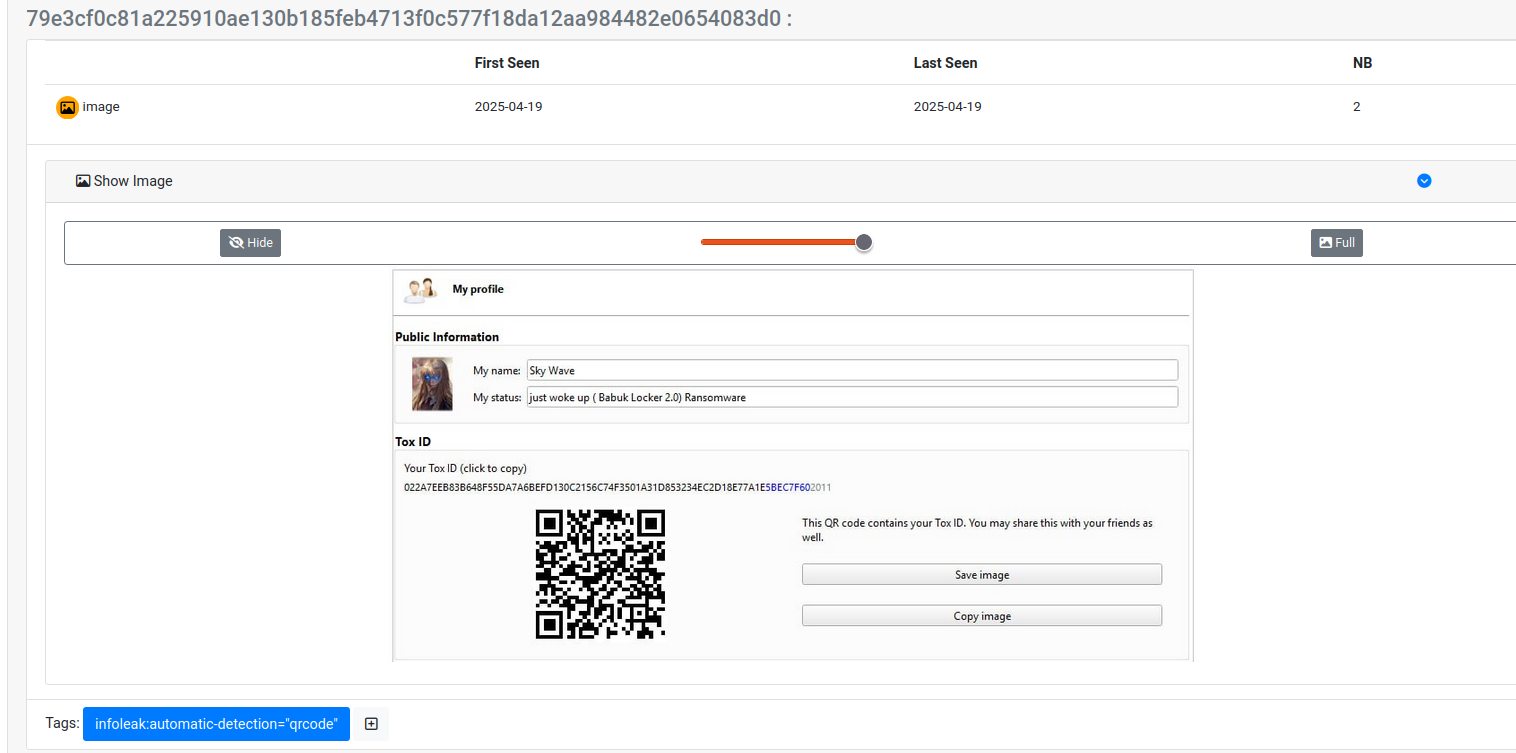
\includegraphics[scale=0.10]{./img/qrcode-3.png}
        \end{column}
        \begin{column}{0.5\textwidth}
            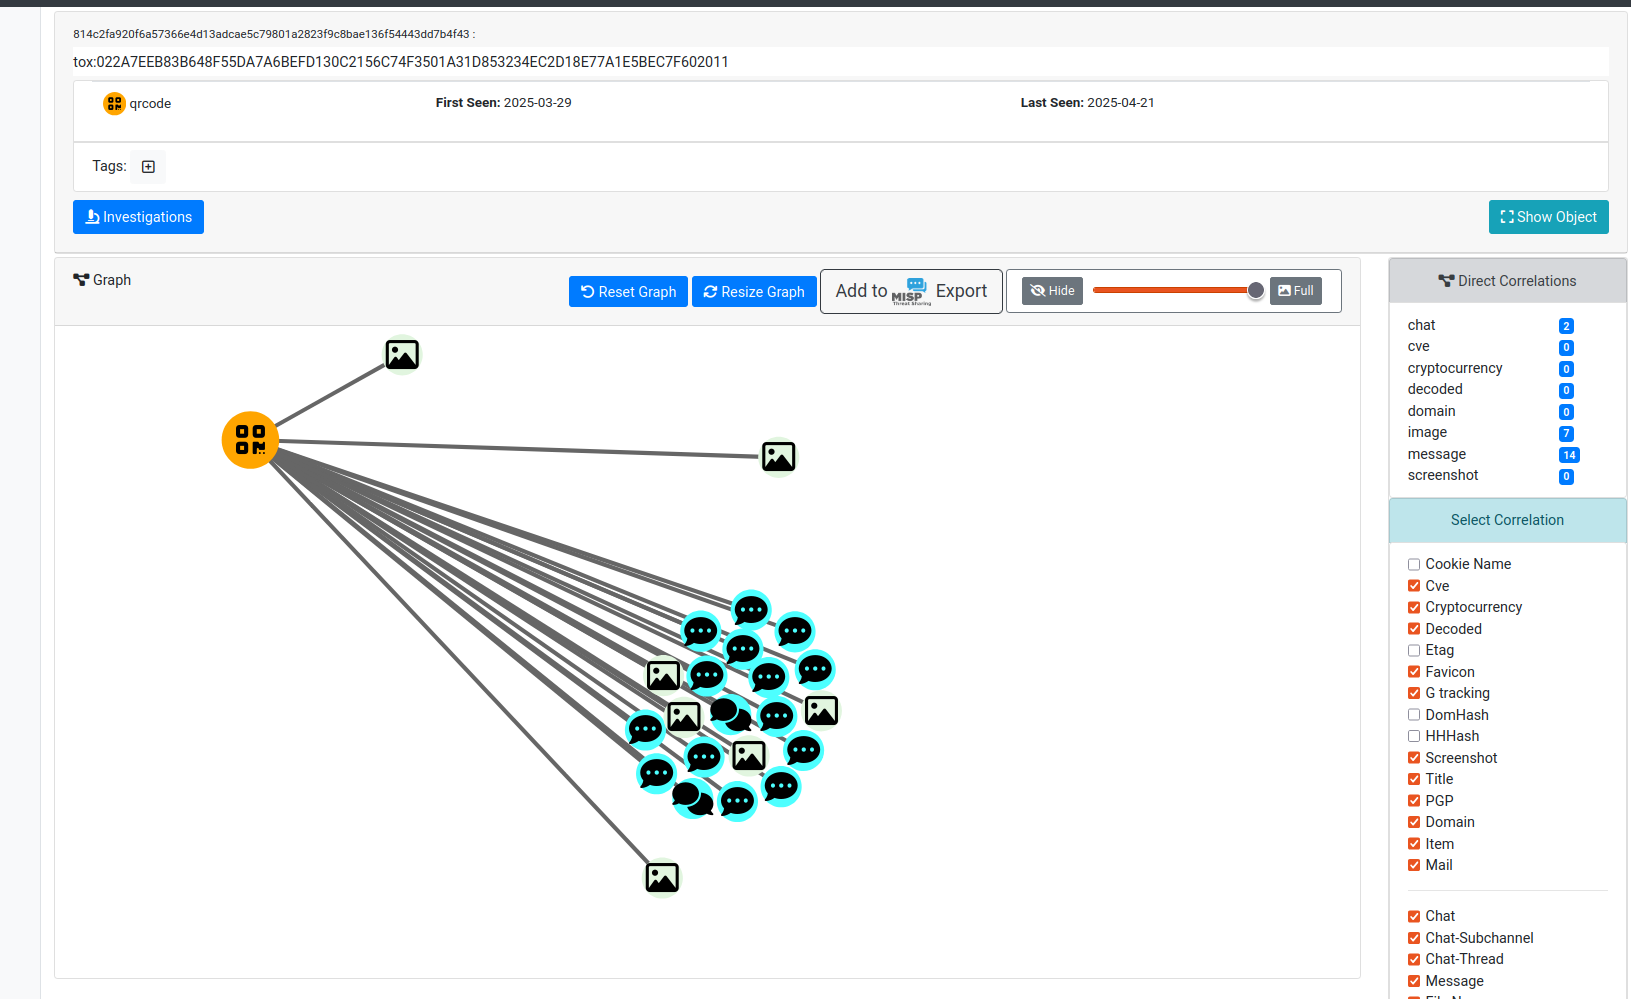
\includegraphics[scale=0.1]{./img/qrcode.png}
        \end{column}
    \end{columns}
\end{frame}

\begin{frame}
    \frametitle{Uncommon Indicator Extraction from Images: Barcodes}
    \begin{itemize}
        \item Following a request from law enforcement, we implemented barcode extraction (Code 128, Code 39, Code 93, etc.).
	\item Barcodes turned out to be {\bf valuable correlation points}, not only in large data leaks, but also in social media interactions involving threat actors.
    \end{itemize}
    \begin{center}
        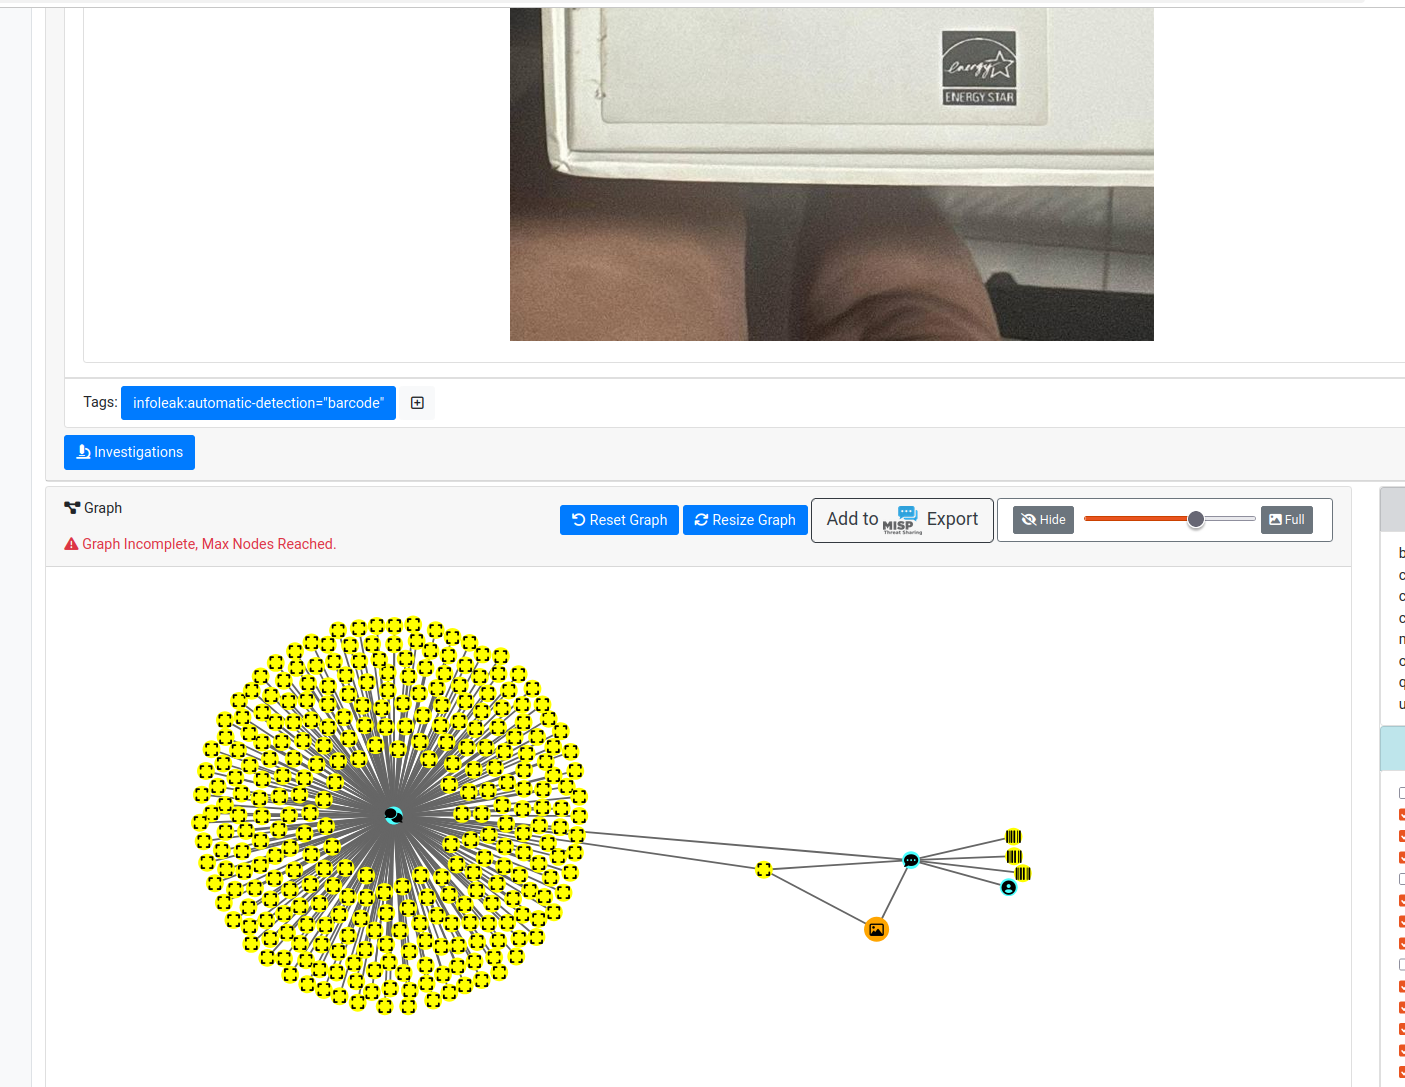
\includegraphics[scale=0.15]{./img/barcode.png}
    \end{center}
\end{frame}

\begin{frame}
    \frametitle{Semantic and Textual Information in Images}
    \begin{itemize}
	    \item {\bf Images often contain valuable textual data}, such as device numbers, identifiers, and embedded messages, that can be extracted for analysis.
        \item CRNN-based OCR models perform well and are highly efficient on modern hardware, making large-scale image parsing feasible.
    \end{itemize}
    \begin{center}
        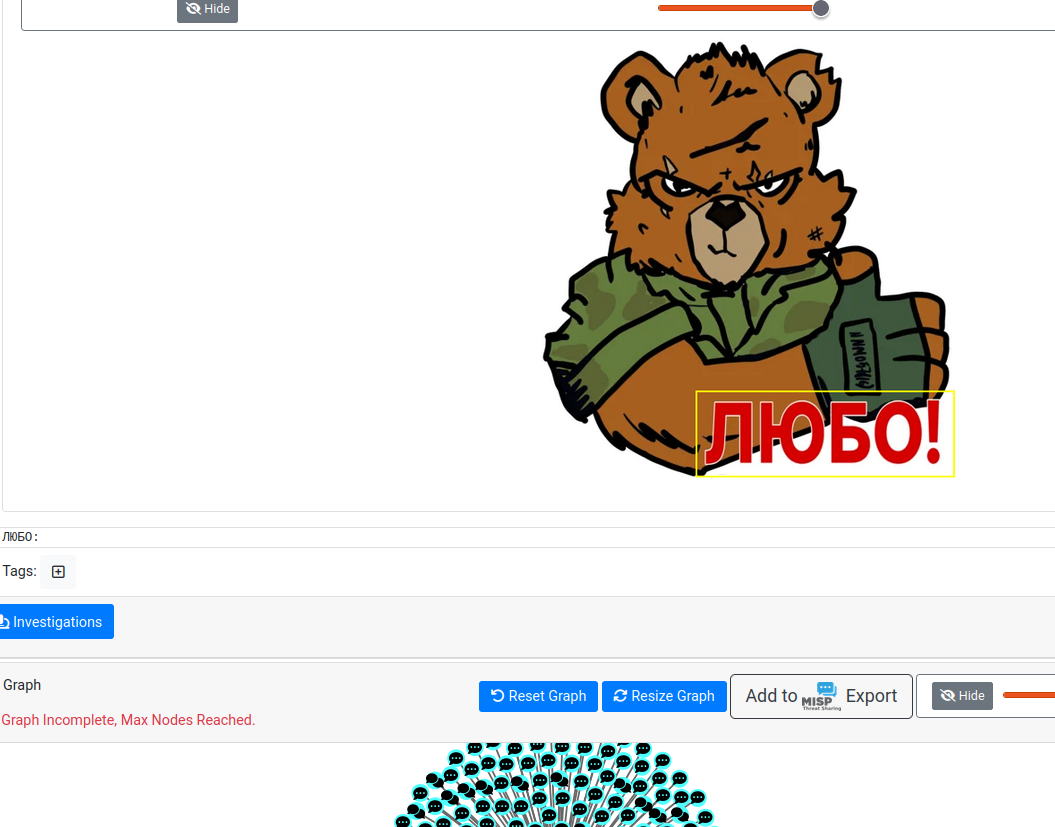
\includegraphics[scale=0.15]{./img/ocr-2.png}
    \end{center}
\end{frame}

\begin{frame}[fragile]
    \frametitle{New Indicators from Common HTML Structures - \texttt{dom-hash}}

    \begin{itemize}
        \item Has everything already been explored in HTML document classification, hashing, or structural similarity detection?
        \item Following a discussion with CERT-PL, we discovered that a {\bf simple strategy yields excellent results}\footnote{Tested against LookyLoo dataset \url{https://lookyloo.circl.lu}} and led to the development of the \texttt{dom-hash} algorithm.
    \end{itemize}

    \vspace{1em}

    \begin{minted}[fontsize=\fontsize{6.5}{8}, bgcolor=bg, tabsize=2]{python}
def _compute_dom_hash(html_content):
    soup = BeautifulSoup(html_content, "lxml")
    to_hash = "|".join(t.name for t in soup.findAll()).encode()
    return sha256(to_hash).hexdigest()[:32]
    \end{minted}

\end{frame}

\begin{frame}
    \frametitle{Fast Clustering of Tor Hidden Services using \texttt{dom-hash}}

    \begin{center}
        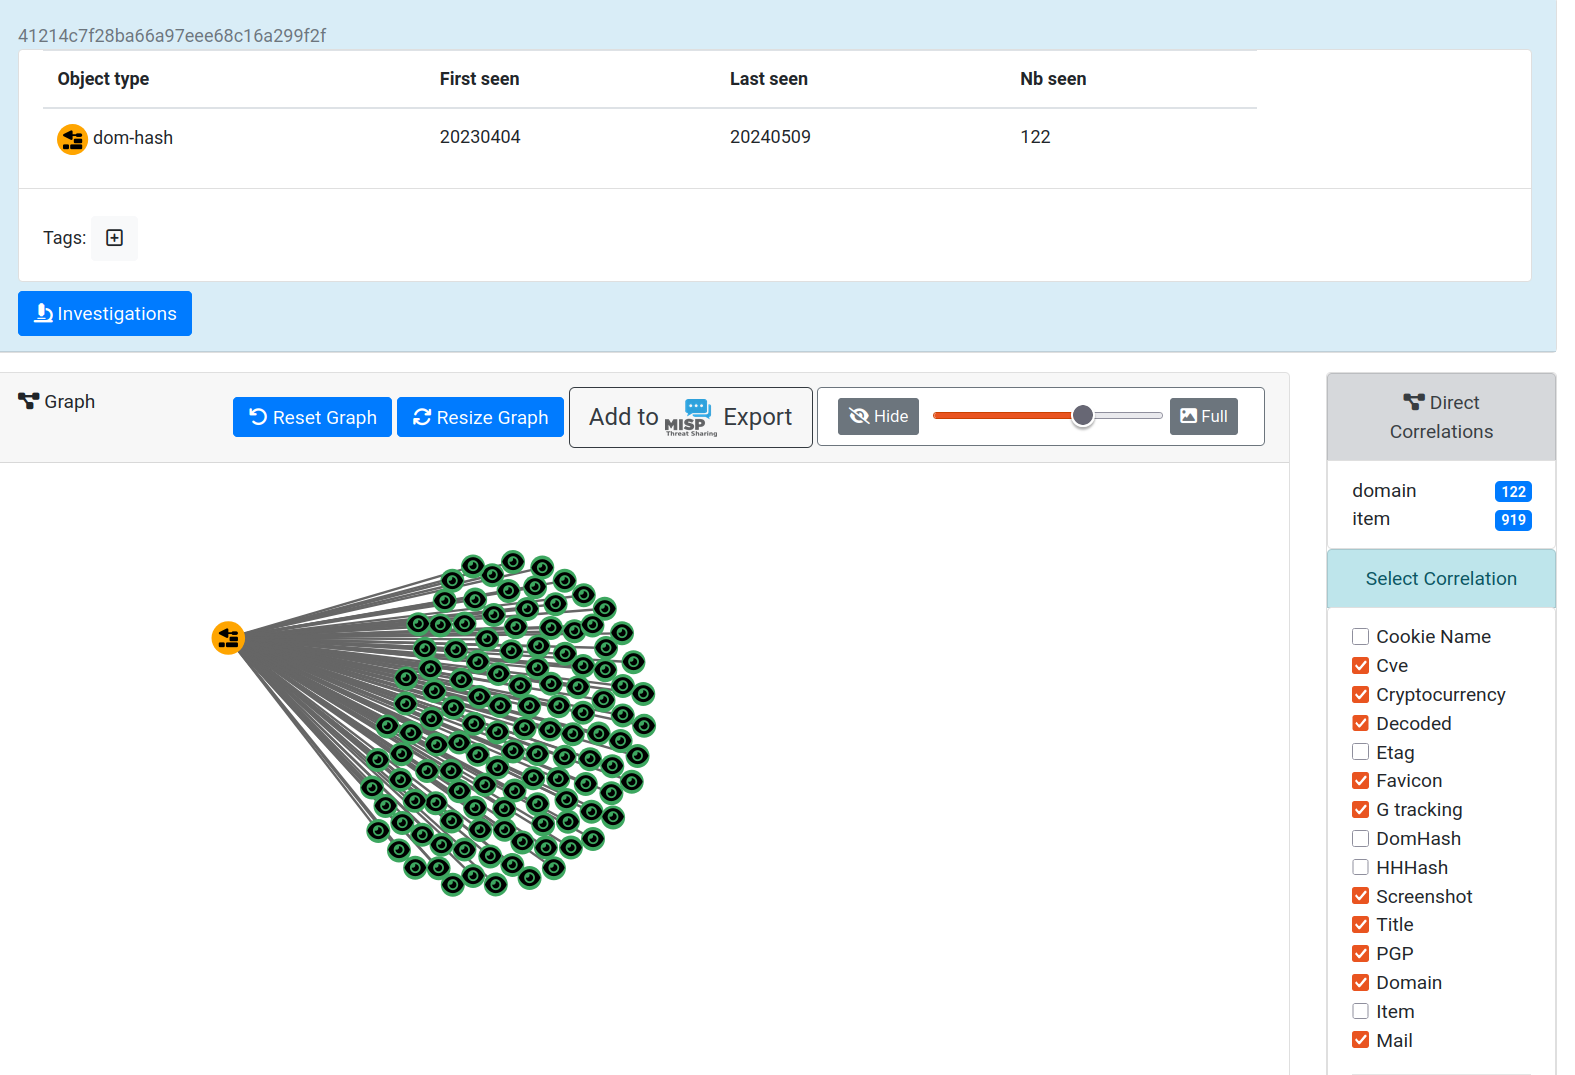
\includegraphics[scale=0.20]{./img/dom-hash.png}
    \end{center}

\end{frame}


\begin{frame}
    \frametitle{What Simple Correlations Are Often Missed? — HTTP Headers}
    \begin{center}
	    HTTP (version 1) response headers can act as subtle fingerprints (HHHash)\footnote{\url{https://www.foo.be/2023/07/HTTP-Headers-Hashing_HHHash}} for linking threat infrastructure.
        \vspace{1em}

        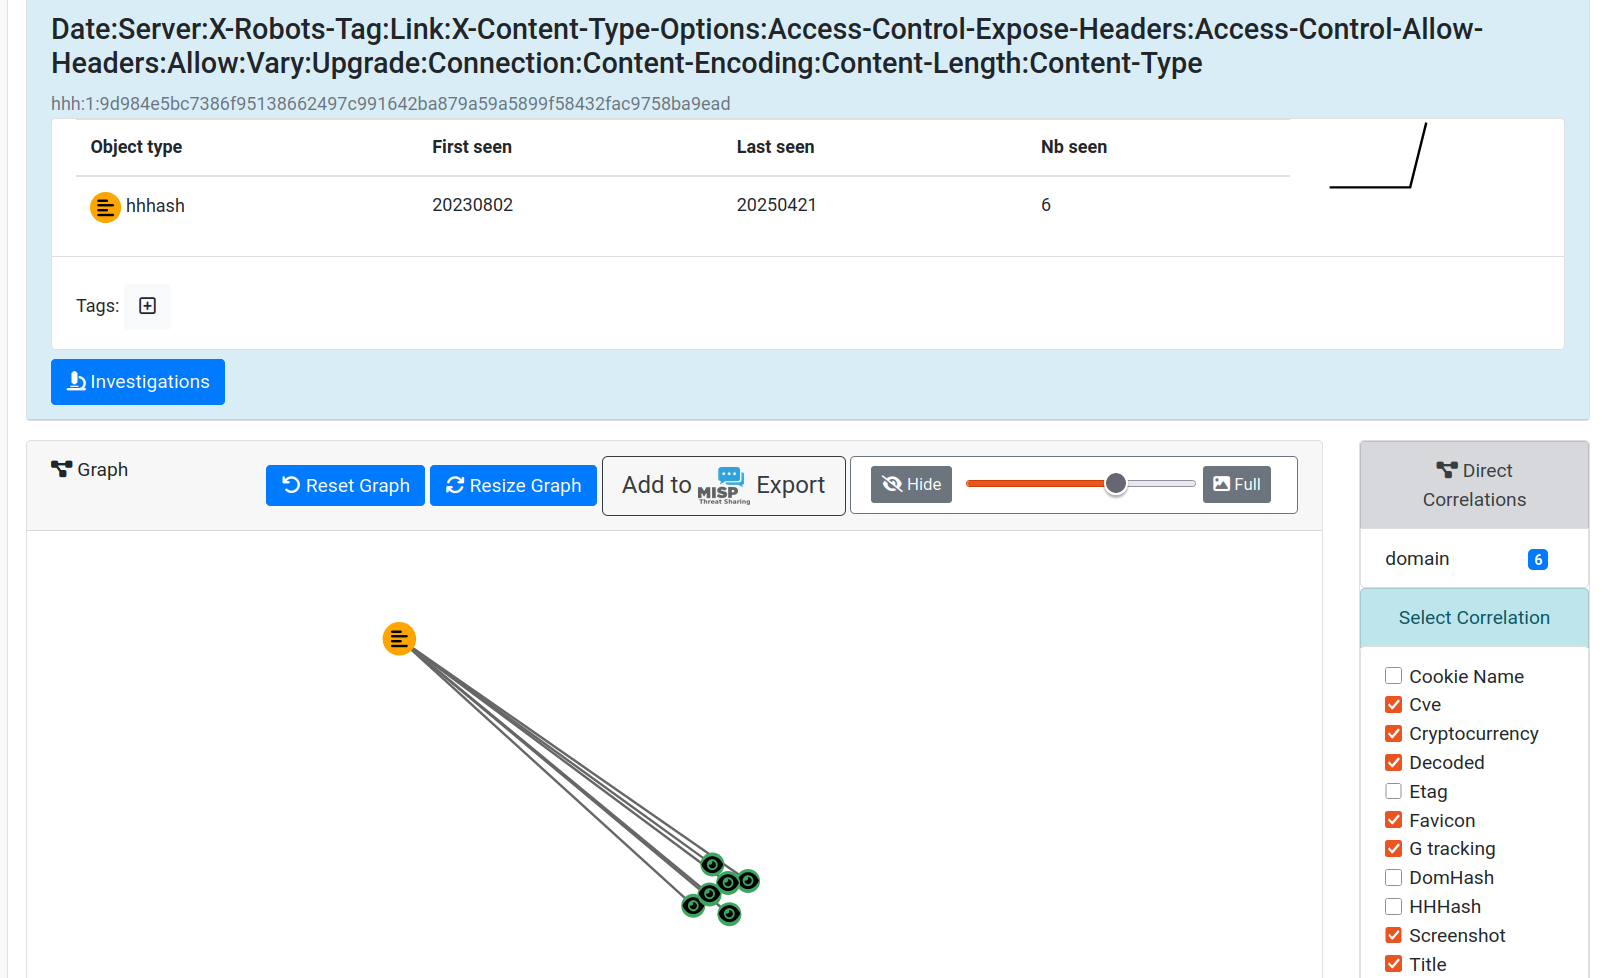
\includegraphics[scale=0.11]{./img/hhh.png}
        \hspace{0.5em}
        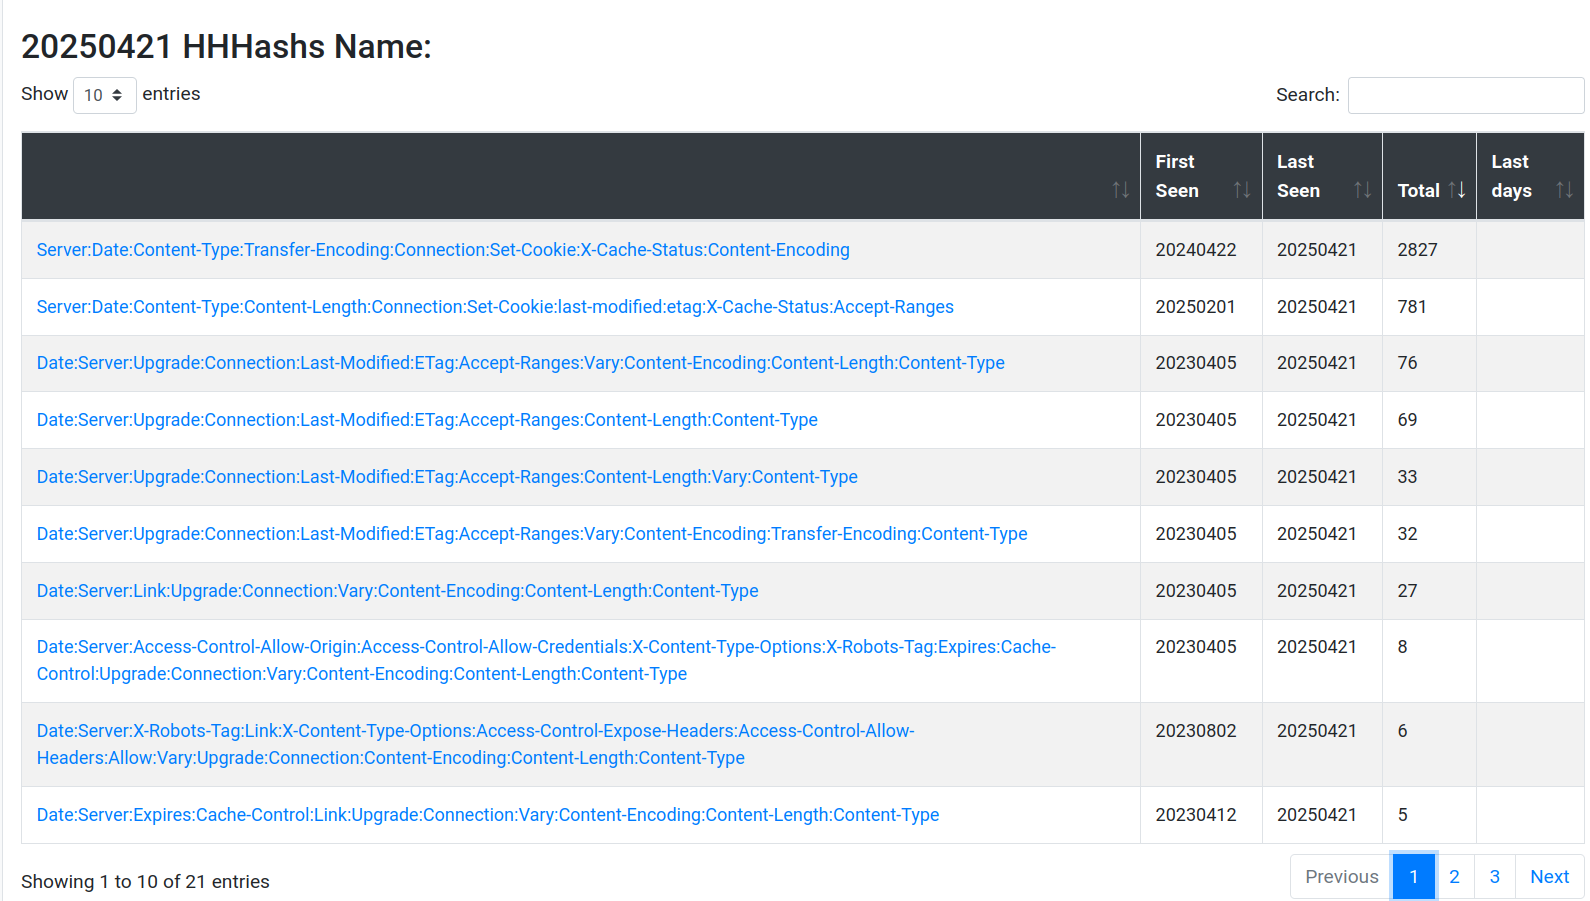
\includegraphics[scale=0.11]{./img/hhh2.png}
    \end{center}
\end{frame}

\begin{frame}
    \frametitle{Another Simple Correlation? — Cookie Names}
    \begin{center}
	\begin{itemize}
		\item Custom or reused cookie names\footnote{The value of the cookie are also interesting but correlation cannot be used as it without further processing} can serve as low-noise indicators for linking {\bf attacker-controlled web infrastructure}.
	\end{itemize}
        \vspace{1em}
        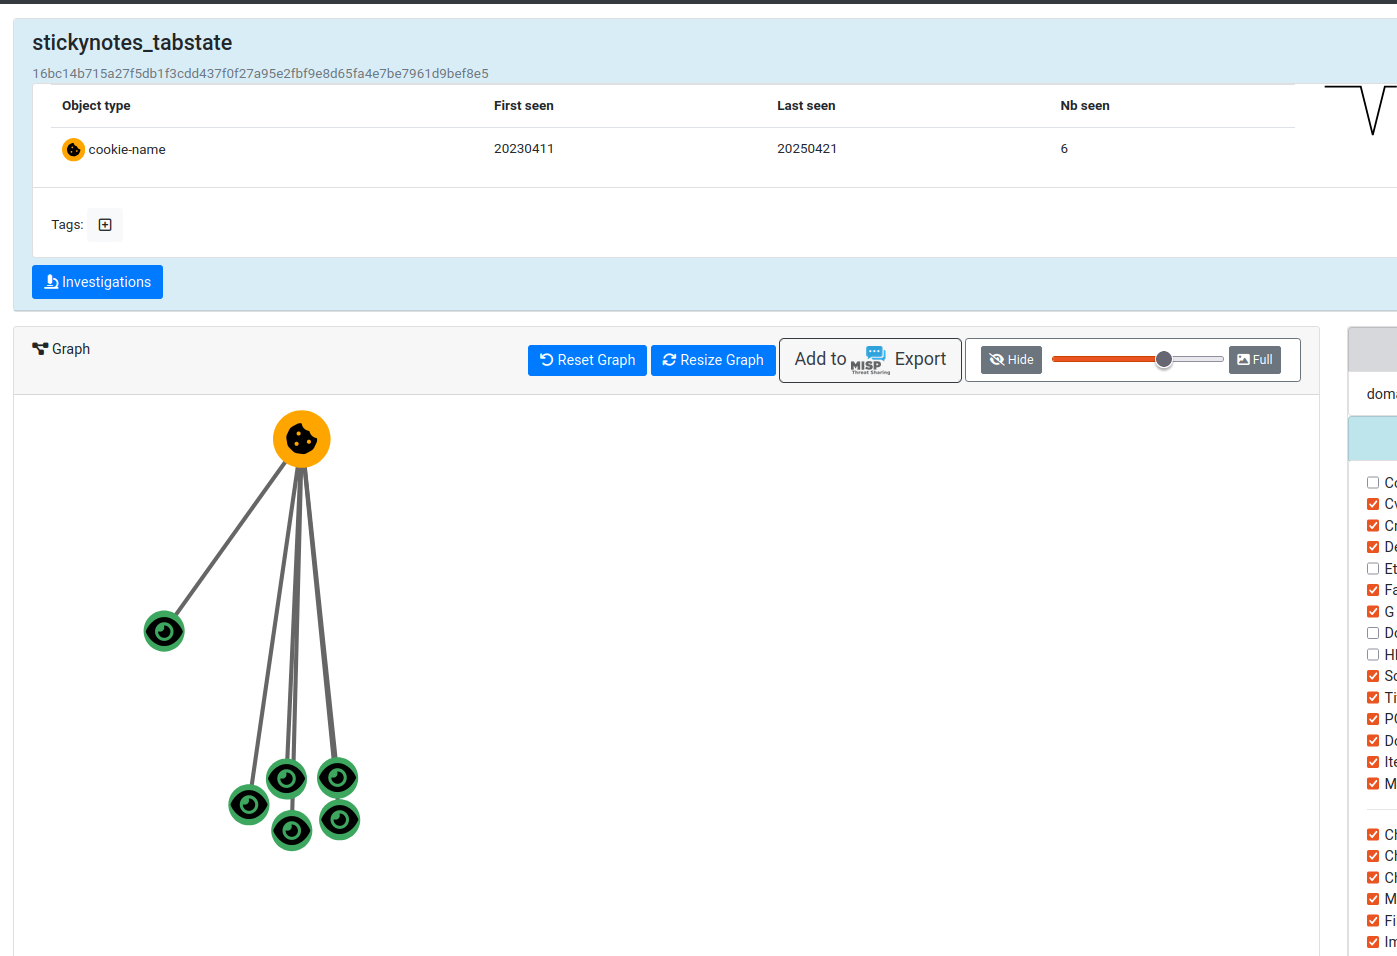
\includegraphics[scale=0.12]{./img/cookies.png}
        \hspace{1em}
        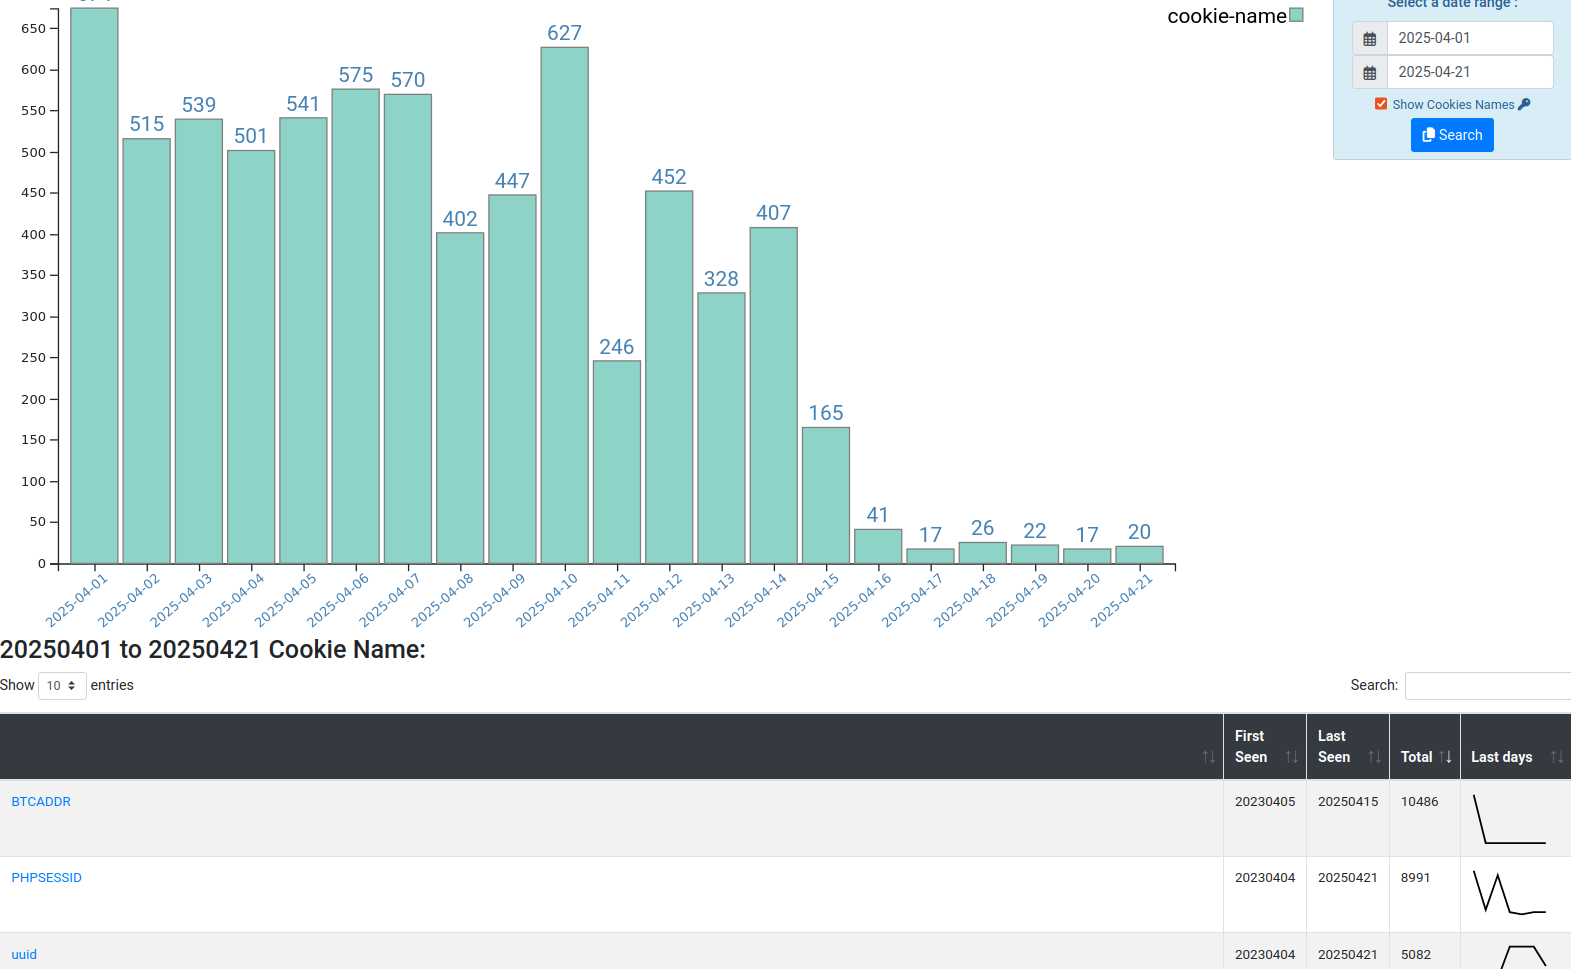
\includegraphics[scale=0.12]{./img/cookies-2.png}
    \end{center}
\end{frame}

\begin{frame}
    \frametitle{An Even Simpler Correlation Indicator? — Filenames}
    \begin{itemize}
        \item In threat intelligence, filenames are often dismissed as unreliable or noisy indicators that may lead to false conclusions.
        \item However, in some cases, especially on social networks or in leak dumps, filenames can carry meaningful context that reveals key aspects of a threat actor's activity.
    \end{itemize}
    \begin{center}
        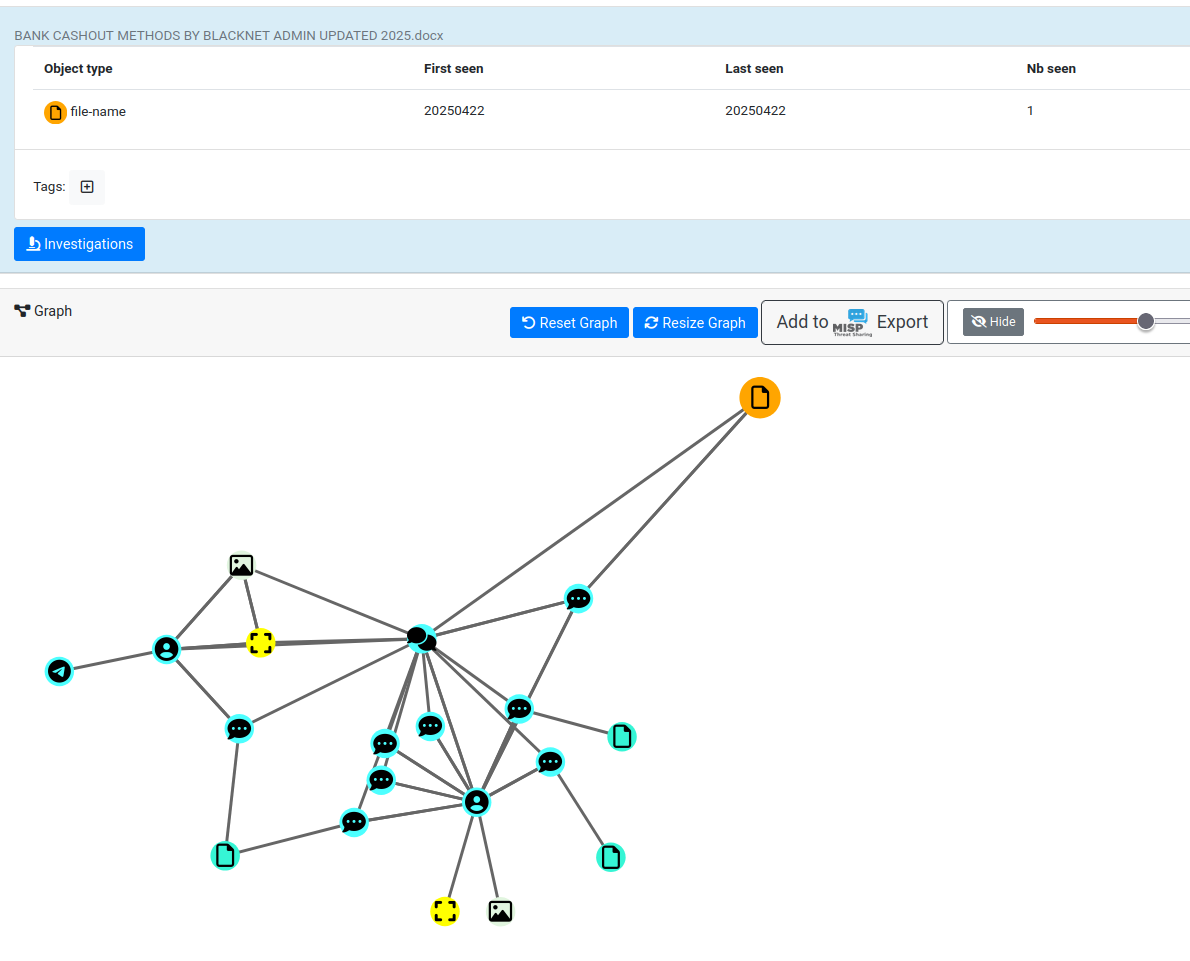
\includegraphics[scale=0.15]{./img/filename.png}
    \end{center}
\end{frame}

\begin{frame}
    \frametitle{Indicators That Threat Actors Should Avoid—But Still Use}
    \begin{itemize}
	    \item It is {\bf commonly assumed that threat actors avoid including labels or metadata} that could link their infrastructure or even their operational teams.
        \item However, our regular crawling of Tor hidden services revealed that Google Analytics tracking codes\footnote{Based on monthly crawling of Tor hidden services, which explains the distribution shown in the graph.} were reused across multiple sites, uncovering unexpected and meaningful correlations.
    \end{itemize}
    \begin{center}
        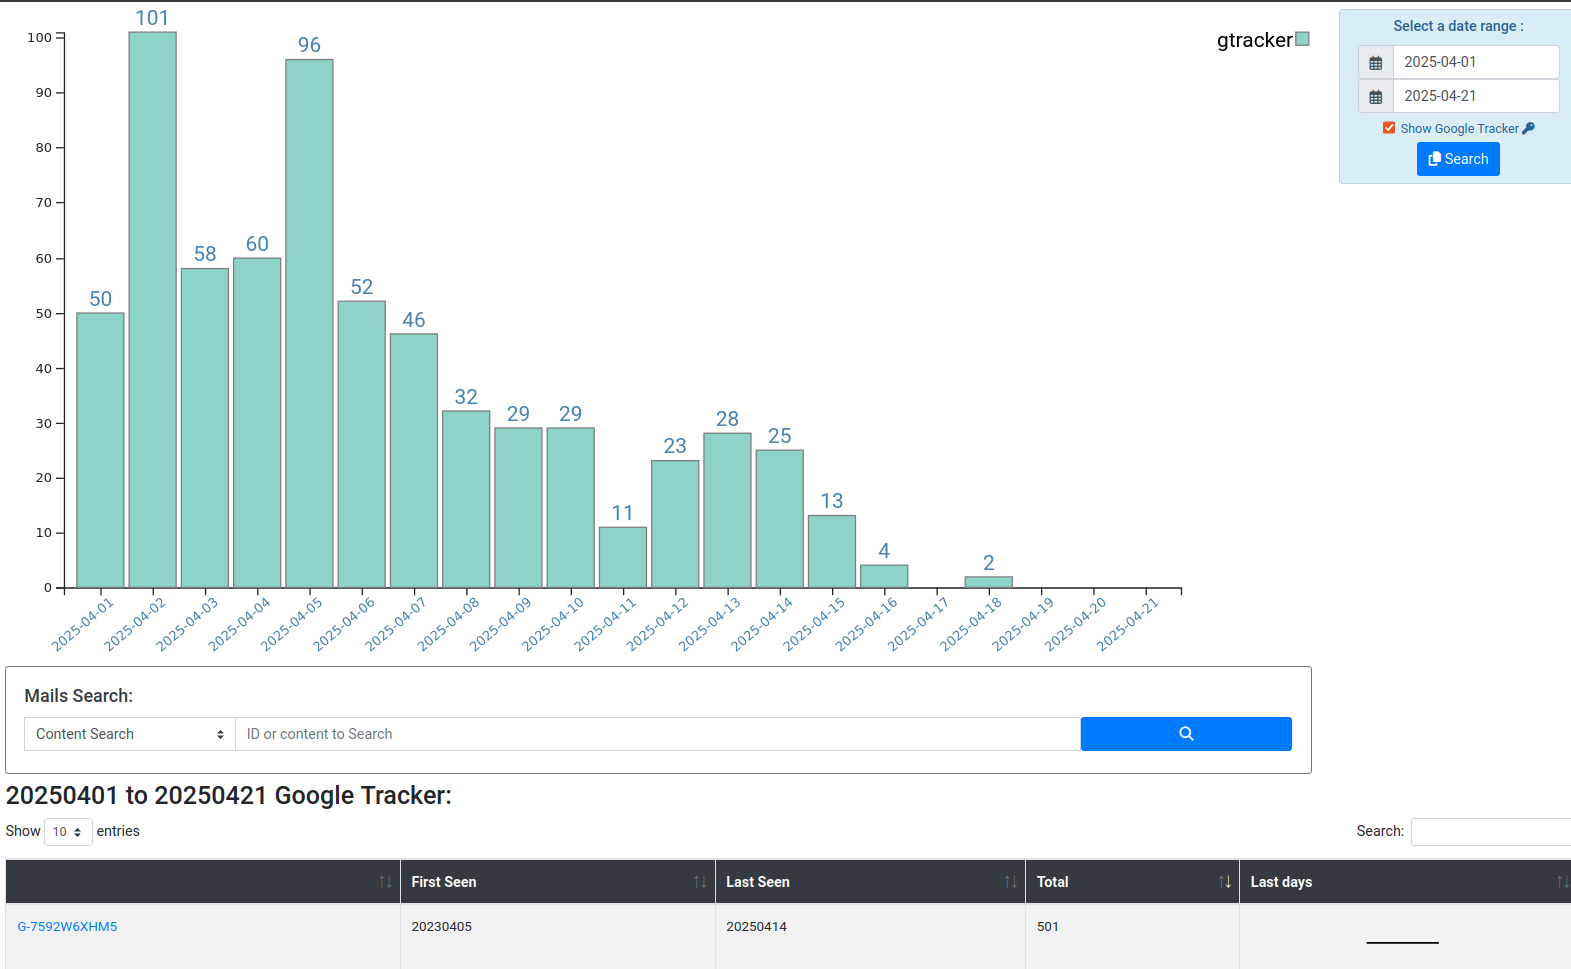
\includegraphics[scale=0.1]{./img/google-trackers.png}
    \end{center}
\end{frame}


\begin{frame}
    \frametitle{Even "Weak" Indicators Like Google Analytics Can Be Powerful in Composite Correlation}
    \begin{columns}
        \begin{column}{0.50\textwidth}
            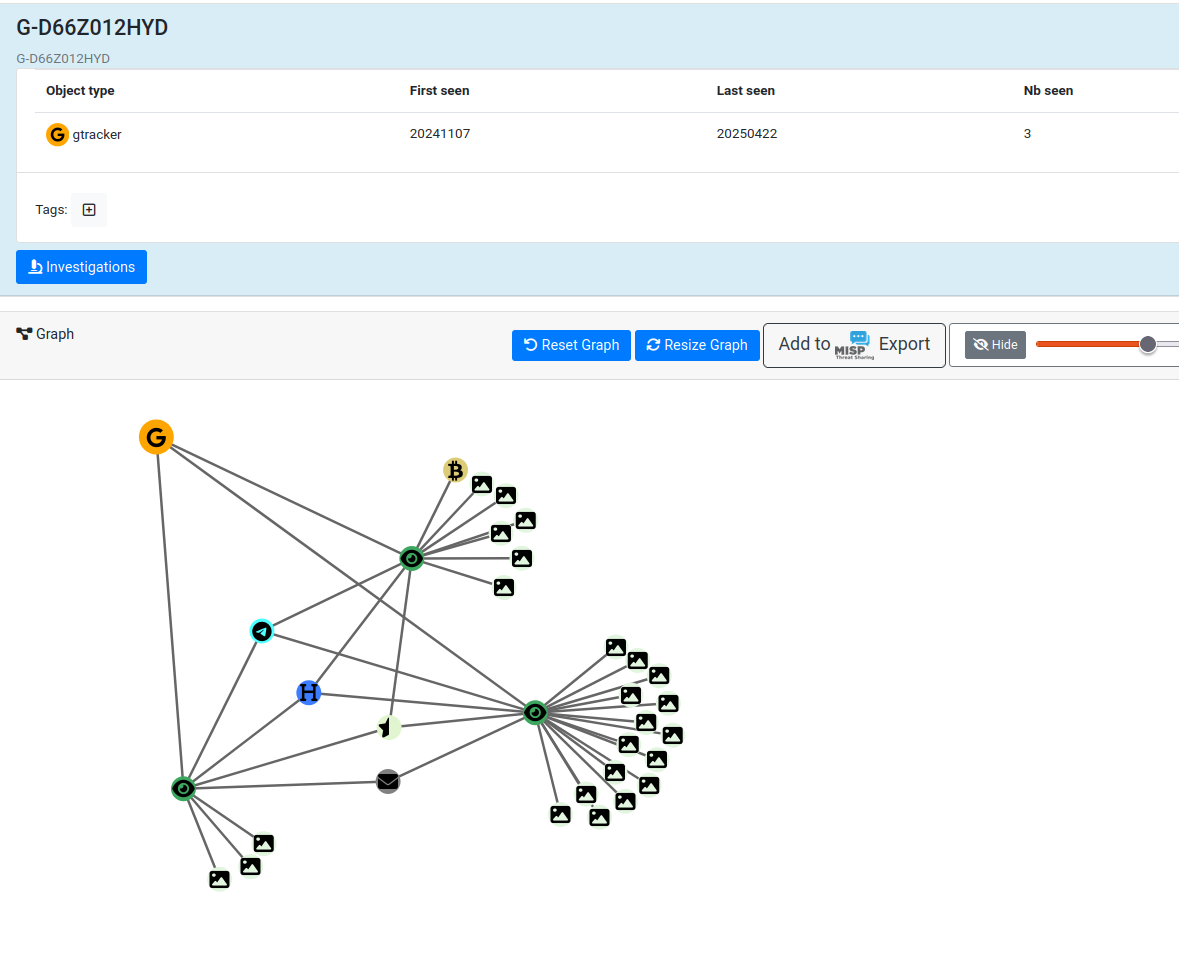
\includegraphics[scale=0.16]{./img/gtracker-2.png}
        \end{column}
        \begin{column}{0.50\textwidth}
            \small
            \textbf{Why it matters:}
            \begin{itemize}
                \item Google Analytics tracking IDs are often reused across phishing domains, malicious sites, or cloned templates.
		\item While GA IDs alone may not prove attribution, when combined with other indicators (e.g., favicon hash, \texttt{dom-hash}, or TLS cert), they help cluster infrastructure belonging to the same threat actor or Tor operator.
                \item Many actors underestimate the traceability of third-party embedded analytics even Ransomware groups.
            \end{itemize}
        \end{column}
    \end{columns}
\end{frame}


\begin{frame}
    \frametitle{Unexpected Correlation from Cryptographic Materials}
    \begin{itemize}
        \item Threat actors often simplify their operations by generating Tor onion services with custom "vanity" addresses—based on recognizable prefixes derived from cryptographic key fingerprints.
	\item While the exact logic behind the generation is not always disclosed, building a tree or graph structure of these vanity addresses can {\bf reveal shared patterns} and uncover related services.
    \end{itemize}
    \begin{center}
        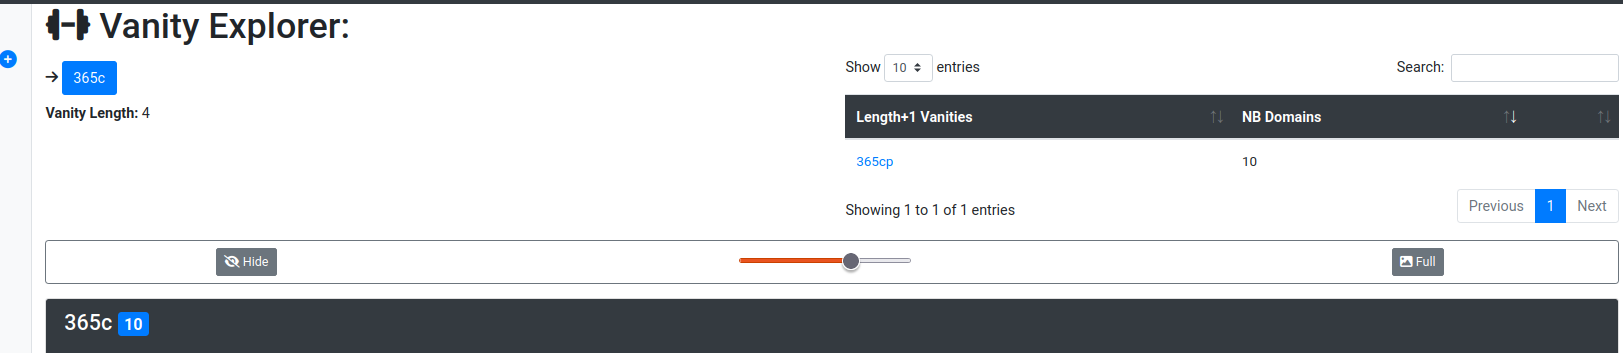
\includegraphics[scale=0.25]{./img/crypto-part.png}
    \end{center}
\end{frame}

\begin{frame}
    \frametitle{Pivoting on Encrypted Messages and Metadata}
    \begin{itemize}
	    \item Sometimes, {\bf collecting encrypted messages or public keys} can reveal unexpected links, especially when metadata is extracted from PGP blocks.
        \item Elements such as key IDs, user IDs, creation dates, or repeated usage of the same key across services can all serve as valuable pivot points.
    \end{itemize}
    \begin{center}
        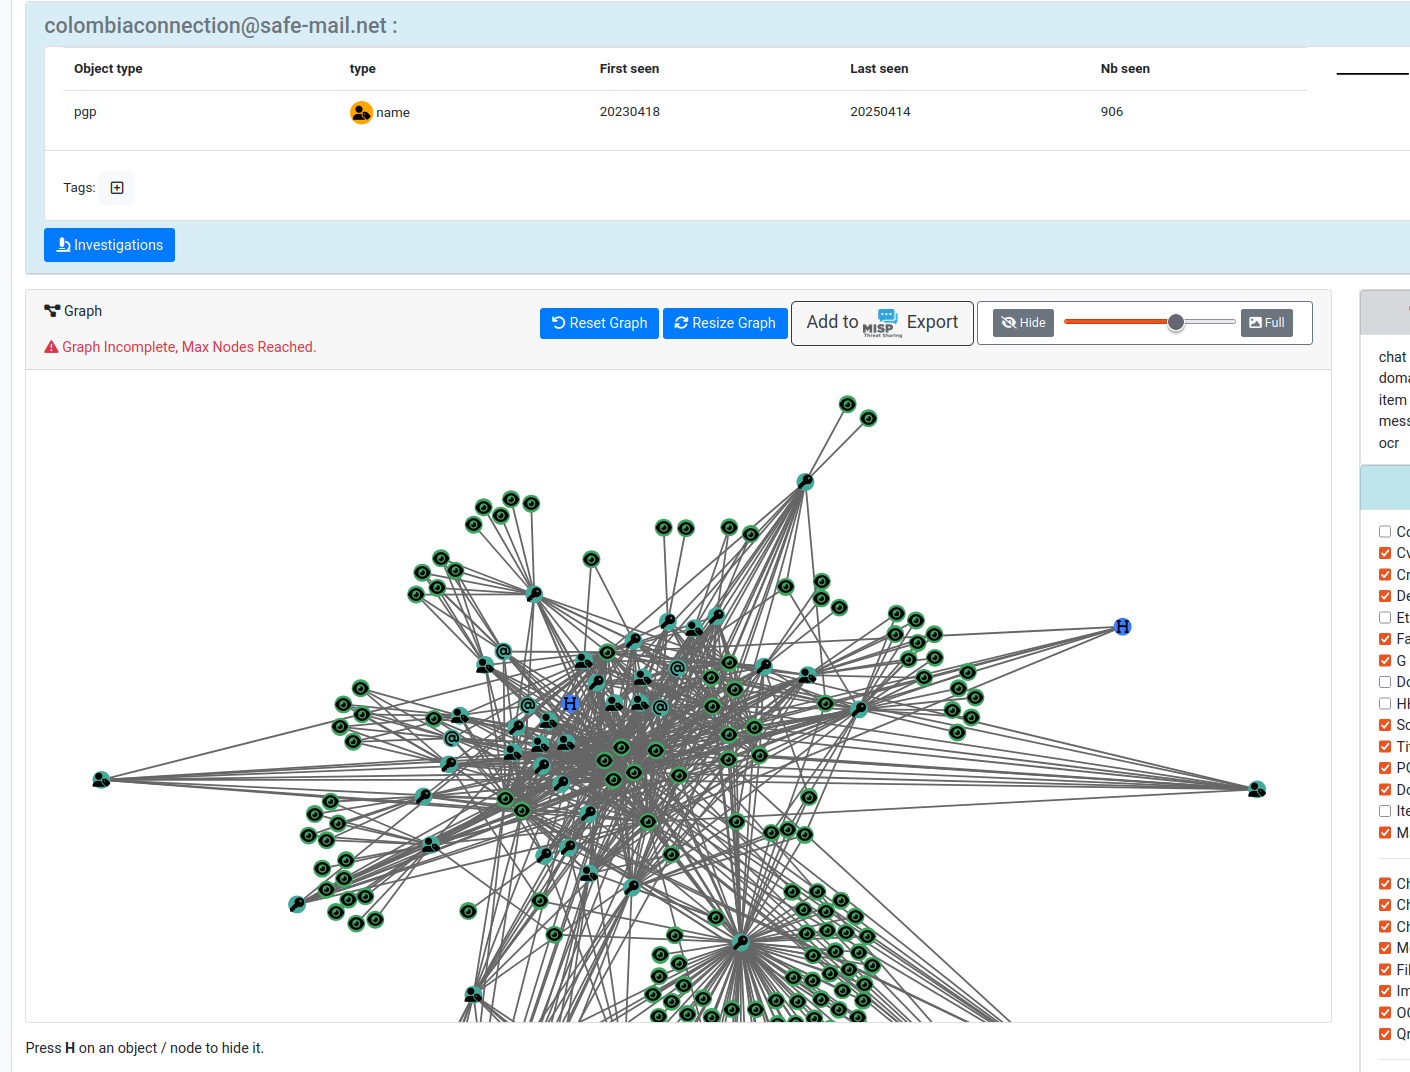
\includegraphics[scale=0.15]{./img/pgp-email.png}
    \end{center}
\end{frame}

\begin{frame}
\frametitle{Passive SSH\footnote{\url{https://github.com/D4-project/passive-ssh}}}
\begin{itemize}
    \item Open‑source \textbf{passive‑ssh} scanner \& database\footnote{\url{https://github.com/D4-project/passive-ssh}}
    \item Captures: public keys, banners, \textbf{hassh} fingerprints
    \item Maintains full host–SSH history (who\,$\rightarrow$\,where, when)
    \item Lean ReST API – lookup by key / hassh / banner
    \item Deanomize onions
    \begin{center}
        
\includegraphics[width=0.2\textwidth]{./img/passivessh.png}
    \end{center}
\end{itemize}
\end{frame}

\begin{frame}
\frametitle{AIL - Passive SSH}
    \begin{center}
        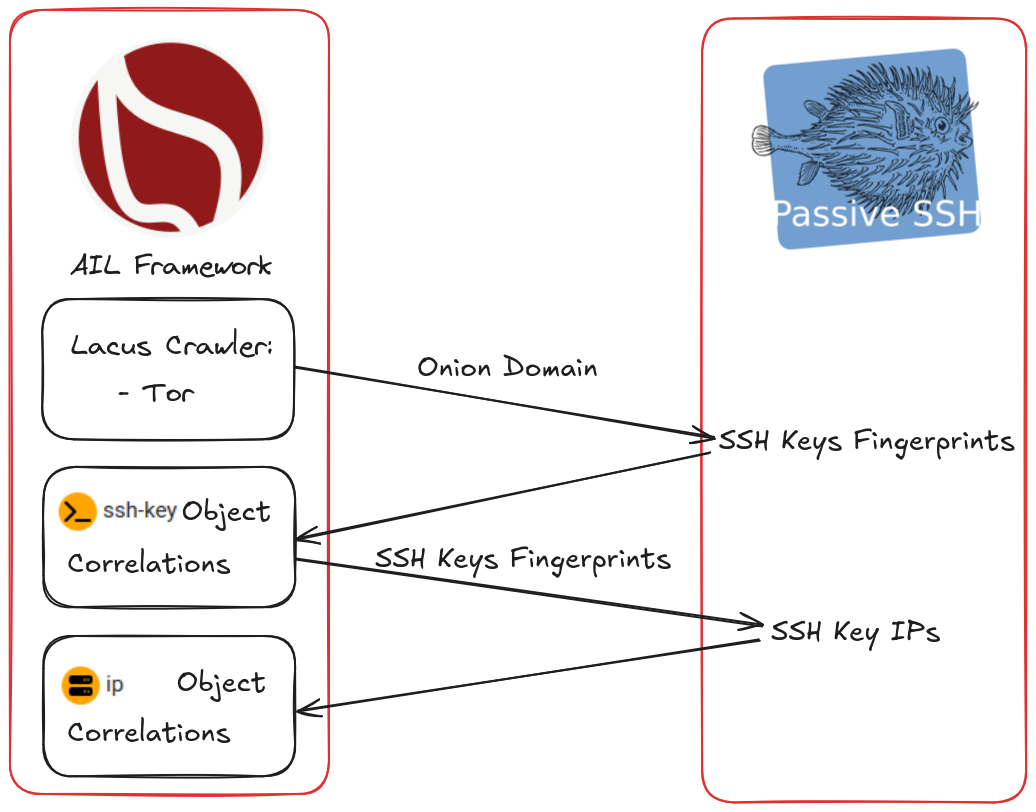
\includegraphics[width=0.65\textwidth]{./img/ssh-crawler.png}
    \end{center}
\end{frame}

\begin{frame}
\frametitle{AIL - SSH Correlation - Shared fingerprints}
    \begin{center}
        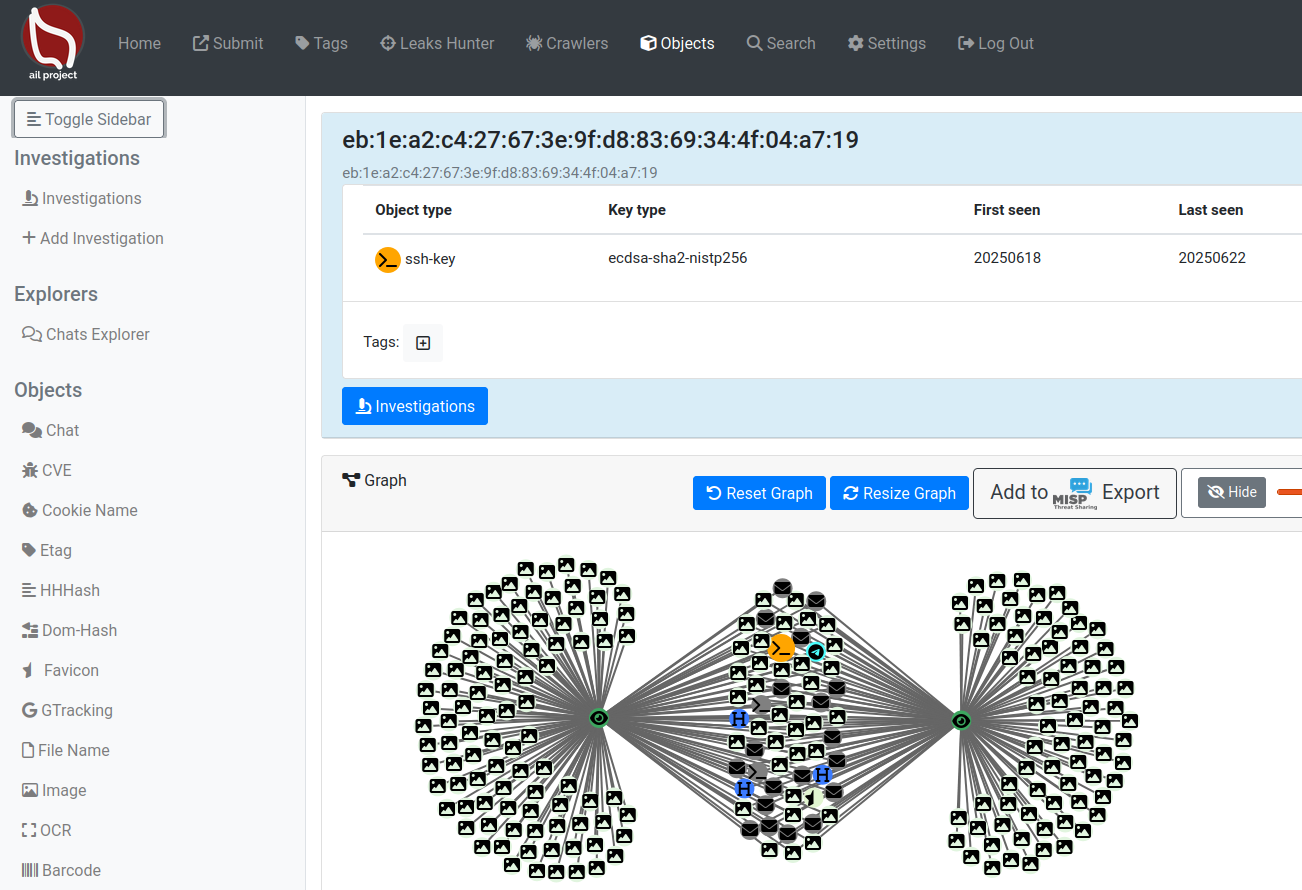
\includegraphics[width=0.8\textwidth]{./img/ail-ssh-correlation-same.png}
    \end{center}
\end{frame}

\begin{frame}
\frametitle{AIL - SSH Correlation - Shared fingerprints}
    \begin{center}
        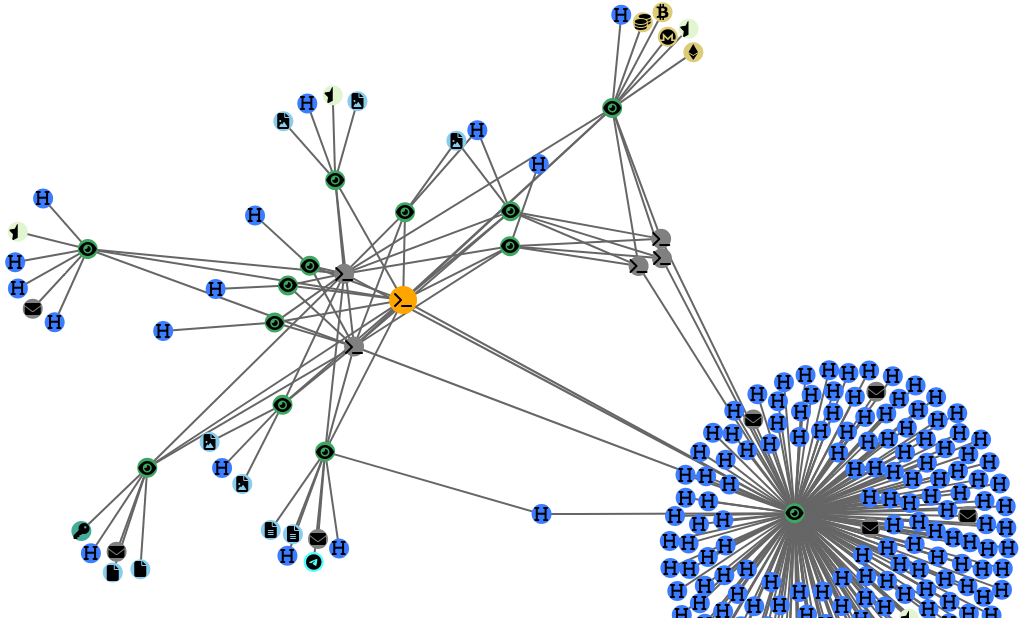
\includegraphics[width=0.8\textwidth]{./img/ail-ssh-correlation.png}
    \end{center}
\end{frame}

\begin{frame}
\frametitle{AIL - Deanomized Onions through shared fingerprints}
    \begin{center}
        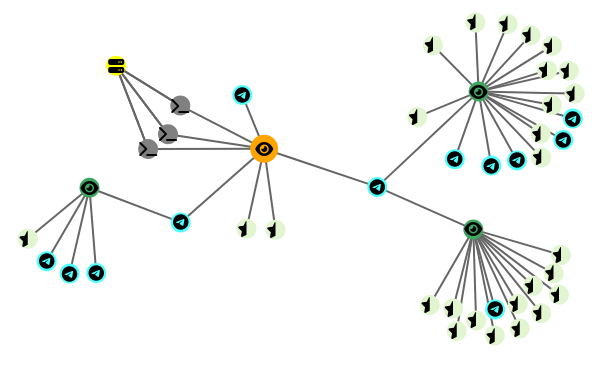
\includegraphics[width=0.8\textwidth]{./img/ail-ssh-deanonimized.png}
    \end{center}
\end{frame}


\begin{frame}
    \frametitle{Conclusion}
    \begin{itemize}
        \item Pivoting is evolving from a manual, intuition-driven process into a reproducible, data-driven discipline—supported by open-source platforms like MISP and AIL.
        \item Uncommon indicators matter just as much as traditional ones, they often reveal what others overlook.
        \item Imperfect doesn’t mean useless. Even outdated or colliding indicators can still provide valuable correlations.
	\item {\bf Creativity is essential}, experimenting with new correlation methods leads to deeper insights and better threat discovery.
    \end{itemize}
\end{frame}

\begin{frame}
	\frametitle{Thank you for your attention}
	\begin{itemize}
		\item AIL project\footnote{All techniques and indicators mentioned in these slides are implemented in the AIL project, using an instance backed by a three-year dataset collected from Tor hidden services and various social networks.}
: \url{https://github.com/ail-project/ail-framework}
		\item For questions, contact: \href{mailto:info@circl.lu}{info@circl.lu}
	\end{itemize}
\end{frame}
\end{document}
